% CVPR 2022 Paper Template
% based on the CVPR template provided by Ming-Ming Cheng (https://github.com/MCG-NKU/CVPR_Template)
% modified and extended by Stefan Roth (stefan.roth@NOSPAMtu-darmstadt.de)

\documentclass[10pt,twocolumn,letterpaper]{article}

%%%%%%%%% PAPER TYPE  - PLEASE UPDATE FOR FINAL VERSION
%\usepackage[review]{cvpr}      % To produce the REVIEW version
\usepackage{cvpr}              % To produce the CAMERA-READY version
%\usepackage[pagenumbers]{cvpr} % To force page numbers, e.g. for an arXiv version

% Include other packages here, before hyperref.
\usepackage{graphicx}
\usepackage{amsmath}
\usepackage{amssymb}
\usepackage{booktabs}


% It is strongly recommended to use hyperref, especially for the review version.
% hyperref with option pagebackref eases the reviewers' job.
% Please disable hyperref *only* if you encounter grave issues, e.g. with the
% file validation for the camera-ready version.
%
% If you comment hyperref and then uncomment it, you should delete
% ReviewTempalte.aux before re-running LaTeX.
% (Or just hit 'q' on the first LaTeX run, let it finish, and you
%  should be clear).
\usepackage[pagebackref,breaklinks,colorlinks]{hyperref}


% Support for easy cross-referencing
\usepackage[capitalize]{cleveref}
\crefname{section}{Sec.}{Secs.}
\Crefname{section}{Section}{Sections}
\Crefname{table}{Table}{Tables}
\crefname{table}{Tab.}{Tabs.}


%%%%%%%%% PAPER ID  - PLEASE UPDATE
\def\cvprPaperID{*****} % *** Enter the CVPR Paper ID here
\def\confName{CVPR}
\def\confYear{2022}


\begin{document}

%%%%%%%%% TITLE - PLEASE UPDATE
\title{Improving Facial Keypoints Detection Through Image Augmentation, Split Pipelining, and Stacked Genrealization of Weak Learners}

\author{Cristopher Benge\\
Columbia University\\
New York, NY\\
{\tt\small cb3704@columbia.edu}
% For a paper whose authors are all at the same institution,
% omit the following lines up until the closing ``}''.
% Additional authors and addresses can be added with ``\and'',
% just like the second author.
% To save space, use either the email address or home page, not both
}
\maketitle

%%%%%%%%% ABSTRACT
%%%%%%%%% ABSTRACT
\begin{abstract}
In this paper, we present a novel approach to improving facial keypoint detection performance by combining image augmentation techniques, stacked generalization of weak learners, and exploitation of diverse training data subsets via targeted splitting of data preparation and training pipelines.  Our methodology entails careful data preprocessing, including thorough cleaning of provided images and labels to ensure high-quality training data is available to all learners.  Further, We leverage a stacked ensemble architecture comprising multiple simple neural networks, each trained on a subset of the data arranged by different data organizers, with a final linear meta-model that utilizes multiplication-based feature interactions for the final prediction.  This approach resulted in a final RMSE of 1.28637, good for second place in a Kaggle competition and only 0.004 RMSE off from a tie for first place.\footnote{Solution available on GitHub: \href{https://github.com/cbenge509/w4732_final_project}{cbenge509 - W4732 Final Project}}

\end{abstract}

%%%%%%%%% INTRODUCTION
%%%%%%%%% INTRODUCTION
\section{Introduction}
\label{sec:intro}

Facial keypoint detection, the task of localizing and identifying key facial landmarks in images, serves as a fundamental component in various computer vision applications such as facial recognition, emotion analysis, and facial expression synthesis. Further, the accurate localization of key facial landmarks such as eyes, nose, and mouth corners is crucial for tasks like face alignment and tracking, enabling advancements in human-computer interaction, biometrics, and augmented reality.  Despite significant advancements in recent years, accurate and robust facial keypoint detection remains a challenging problem due to variations in facial expressions, poses, lighting conditions, and occlusions.~\cite{WANG201850} \\

Traditional approaches to facial keypoints detection often rely on handcrafted features and shallow learning models, which may struggle to capture the complex and subtle patterns present in facial images or generalize well to diverse and complex datasets. With the emergence of deep learning, convolutional neural networks (CNNs) have demonstrated remarkable success in automatically learning hierarchical representations directly from raw pixel data.~\cite{9065279}  However, the success of CNN-based methods heavily depends on the quality and diversity of the training data, as well as the effectiveness of the training process itself.\\

In this paper, we propose a novel approach to enhancing facial keypoints detection performance by integrating several key strategies: image correction and label fine-tuning, stacked generalization of weak learners leveraging a K-fold strategy, and a split pipeline for data processing and training through detection of individual contributing organizers, allowing for exploitation of variance in labeling patterns. To further enhance the robustness of our system, we incorporate image augmentation techniques, artificially expanding the training dataset, thereby improving diversity and generalized performance of each weak learner.\\

To evaluate the effectiveness of our approach, we conduct extensive experiments on a benchmark facial keypoints detection dataset from the 2017 Kaggle competition: \href{https://www.kaggle.com/competitions/facial-keypoints-detection/overview}{Facial Keypoints Detection}.  Competition submissions are scored on the root mean squared error as the standard metric for comparing solution quality:
\begin{equation}
	\text{RMSE} = \sqrt{\frac{1}{N} \sum_{i=1}^N \left(y_i - \hat{y}_i\right)^2}
\end{equation}
Our results demonstrate that the proposed method achieves state-of-the-art performance. Overall, this paper presents a comprehensive framework for improving facial keypoints detection, offering valuable insights into the synergy between data augmentation, ensemble learning, and data processing techniques in the context of computer vision tasks.

%-------------------------------------------------------------------------
\subsection{Related Work}

Facial keypoint detection has been a subject of active research in computer vision for several decades, with a variety of approaches proposed.  Traditional methods often relied on handcrafted features and shallow learning models, such as support vector machines (SVMs) coupled with techniques like Haar cascades or local binary patterns (LBP) for feature extraction~\cite{VIOLAANDJONES2014, 1717463}. \\

In recent years, the rise of deep learning has transformed facial keypoints detection work by enabling end-to-end learning directly from raw (lcalized) pixel data.  CNNs have emerged as the dominant architecture for this task due to their ability to automatically learn hierarchical representations, capturing both low-level features like edges and high-level semantic information~\cite{LECUN2015NATURE}.  Early CNN-based approaches demonstrated promising results on facial keypoints detection tasks, insporing subsequent research in the domain.~\cite{10.1007/978-3-319-10599-4_7} \\

Several studies have focused on enhancing the robustness and accuracy of facial keypoints detection by exploring various aspects of deep learning architectures and training methodologies.  Zhang et al.~\cite{Zhang_2015} introduced a multi-task learning framework that jointly predicts facial keypoints and facial attributes, leveraging shared representations to improve performance. Similarly, Sun et al.~\cite{6619290} proposed a cascaded CNN architecture that refines keypoints predictions iteratively, enabling better handling of occlusions and variations in facial expressions.\\

Ensemble learning techniques have also been applied to facial keypoints detection, aiming to leverage the diversity of multiple models to improve overall performance. Zhang et al.~\cite{wu2017robust} proposed a boosting-based approach that combines weak learners trained on different subsets of the data, effectively reducing generalization errors and enhancing robustness to outliers.  Similarly, Liu et al.~\cite{liu2015deep} explored the use of stacked generalization, combining predictions from multiple base models with a meta-learner to achieve superior performance.\\

While these prior works have made significant contributions to the field, they often focus on individual aspects of the facial keypoints detection pipeline, such as model architecture or training strategy, without fully exploiting the potential synergy between different techniques.  In contrast, our proposed method integrates image augmentation, stacked generalization, and targeted data preprocessing to achieve state-of-the-art performance, highlighting the importance of a holistic approach to addressing the challenges of facial keypoints detection.\\

\begin{figure}[t]
	\centering
	%\fbox{\rule{0pt}{2in} \rule{0.9\linewidth}{0pt}}
	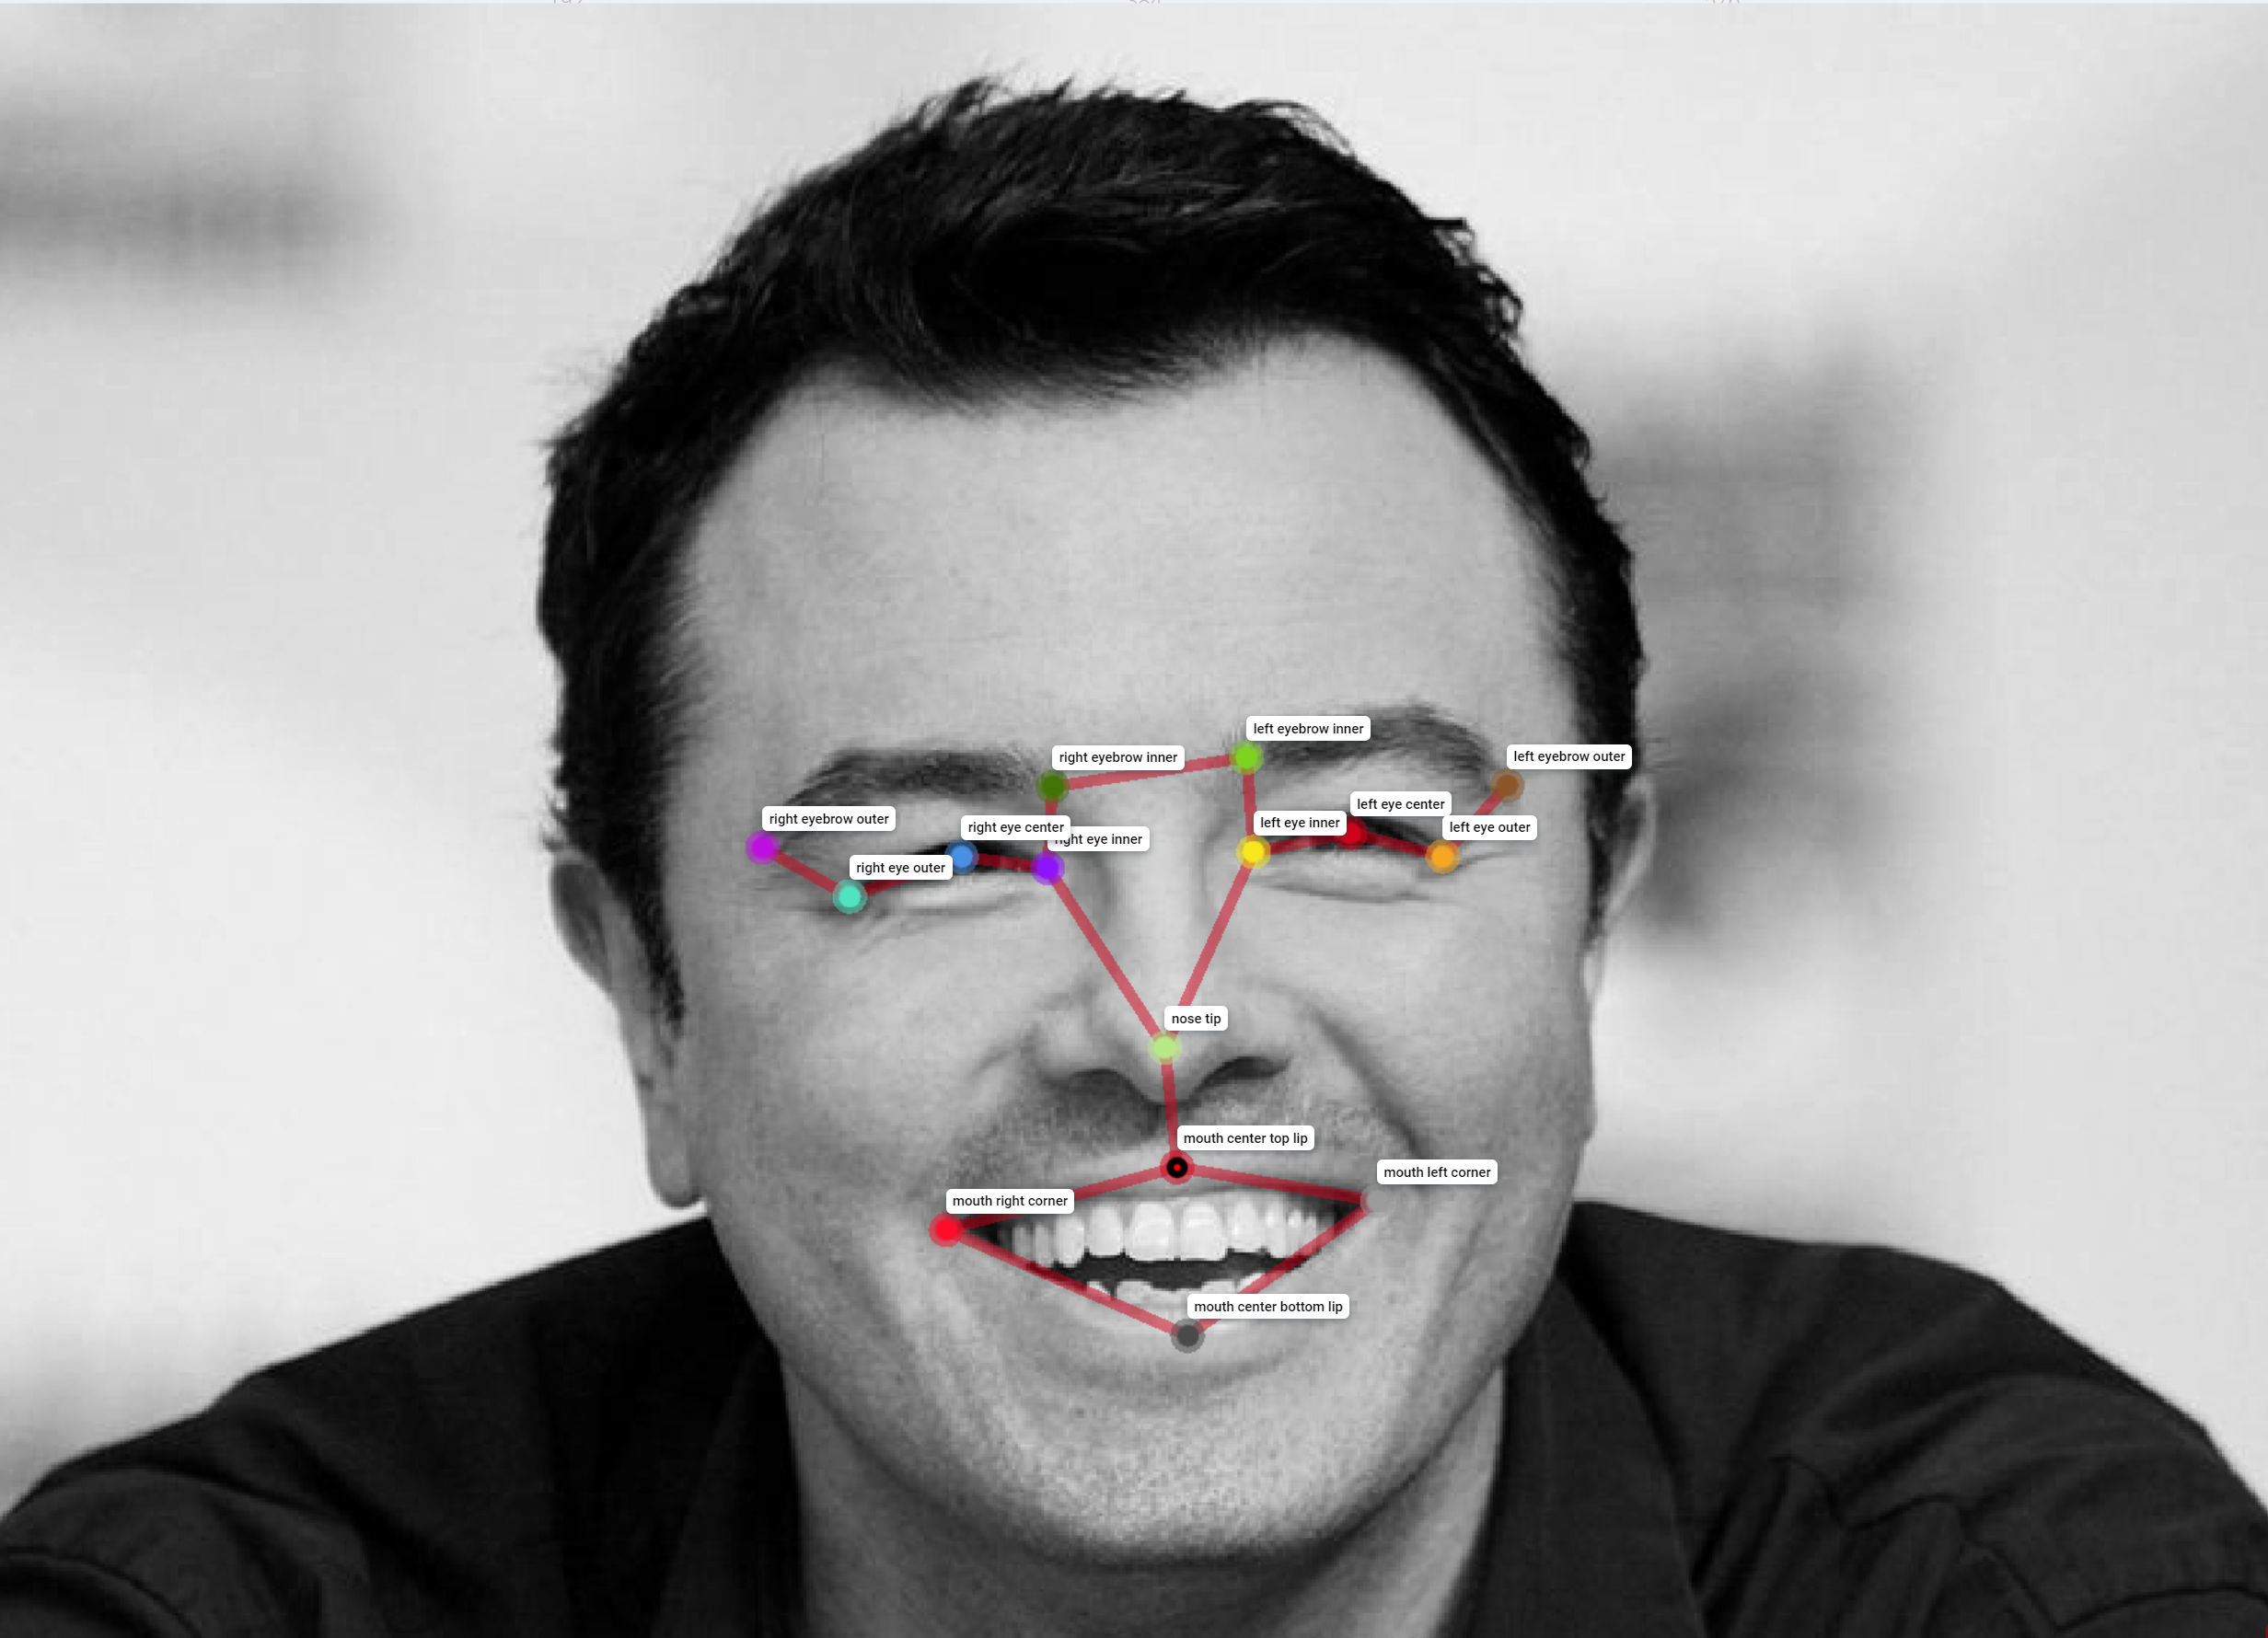
\includegraphics[width=0.95\linewidth]{images/seth.png}
	\caption{Example of 15 facial landmarks labeled on American actor and animator Seth MacFarlane.  This image was not a part of the competition training or test data; rather, it was created to serve as an exemplar inference outcome of our solution.}
	\label{fig:oneexample}
\end{figure}

%%%%%%%%% METHODOLOGY
%%%%%%%%% METHODOLOGY
\section{Methodology}
\label{sec:methodology}

Our proposed methodology for enhancing facial keypoints detection encompasses a comprehensive framework that integrates several aforementioned strategies: image correction and label fine-tuning, stacked generalization of weak learners leveraging a K-fold $(K=5)$ strategy, and a split pipeline for data processing and training through detection of individual contributing organizers, allowing for exploitation of variance in labeling patterns. The following sections outline each component of our methodology in detail.

\begin{figure*}
	\centering
	\begin{subfigure}{0.49\linewidth}
		%\fbox{\rule{0pt}{2in} \rule{.9\linewidth}{0pt}}
		\includegraphics[width=0.99\linewidth]{images/train\_pipeline.png}
		\caption{Training pipeline consists of splitting on partial and complete keypoint examples, training eight separate learners twice (once for each split set), performing generalized stacking on K-flod strategy, and emitting predictions for level-2 metaregressor.}
		\label{fig:short-a}
	\end{subfigure}
	\hfill
	\begin{subfigure}{0.49\linewidth}
		%\fbox{\rule{0pt}{2in} \rule{.9\linewidth}{0pt}}
		\includegraphics[width=0.99\linewidth]{images/inference\_pipeline.png}
		\caption{Inferencing works much the same as our training pipeline, with prediction patterns being split on asks for 15 or 4 labels, generating predictions for each weak learner, and merging those predictions into a single output for input into our level-2 metaregressor.}
		\label{fig:short-b}
	\end{subfigure}
	\caption{Our solution training and inference pipeline that results in state-of-the-art performance for facial keypoints detection.}
	\label{fig:fig2}
\end{figure*}

\subsection{Data Preprocessing and Augmentation}

Prior to model training, we perform extensive data preprocessing to improve quality of labels.  Following extensive exploratory data analysis, we performed the following pre-processing steps:
\begin{itemize}
	\vspace{-0.2em}\item Removal of two training images that did not contain faces or facial keypoint labels.
	\vspace{-0.8em}\item 56 images had incorrect keypoint labels.  All received manually corrected labels to establish a better ground truth.
	\vspace{-0.8em}\item 277 duplicate images identified through hashing; labels were mean averaged and duplicates images removed to reduce bias.
	\vspace{-0.8em}\item 186 images were dropped due to containing neither all nor only-four keypoints (8 labels). This distinction is how we differntiate our split pipeline later.
	\vspace{-0.8em}\item all pixel values were normalized $(\bar{x} = \frac{x}{255})$
\end{itemize}

\pagebreak

To augment the training dataset and improve model generalization, we employ various image augmentation techniques. These include positive and negative rotations, elastic transformation of images, injection of random gaussian noise, brightening and dimming, constrast stretching, image sharpening, horizontal flipping, and Contraste Limited AHE (\href{https://en.wikipedia.org/wiki/Adaptive_histogram_equalization}{adaptive histogram equalization}).  This process, outlined in \cref{fig:datapipeline} below, produced an 18-fold increase in training data available to our weak learners.

\begin{figure}[h]
	\centering
	%\fbox{\rule{0pt}{2in} \rule{0.9\linewidth}{0pt}}
	\includegraphics[width=0.95\linewidth]{images/data\_augmentation\_pipeline.png}
	\caption{Data augmentation pipeline results in 18x training images and better generalization.}
	\label{fig:datapipeline}
\end{figure}

\subsection{Stacked Generalization of Weak Learners}

Our methodology adopts a stacked ensemble architecture~\cite{WOLPERT1992241}, which combines predictions from multiple weak learners to make final predictions. We employ a K-fold strategy to divide the dataset into training and validation sets, ensuring that each model is trained on a diverse subset of the data and evaluated on unseen samples. Predictions of the held-out values are saved to train the final level-2 metaregressor after multiplication-based feature interactions are generated.  See \cref{fig:kfoldstacking} for depiction of this process.

We evaluated dozens of simple neural network architectures for individual performance and eliminate those that either under-perform or have predictions with a high pearson correlation to another model already included in our ensemble. Resultingly, sevel models were chosen as final candidates for our level-1 weak learners.  See \cref{tab:sevenmodels}.

\begin{table}
	\raggedright
	\centering
	\small
	\begin{tabular}{p{2.3cm}|p{5.7cm}}
		\toprule
		\textbf{Model} & \textbf{Description} \\
		\midrule
		Conv2D 5-layer & A simple 5-layer 2d CNN. \\
		\midrule
		NaimishNet & A 7.4M parameter 2D CNN that learns only one keypoint at a time (\href{https://arxiv.org/abs/1710.00977}{paper}). \\
		\midrule
		Conv2D 10-layer & A deeper version of Conv2D 5-layer above. \\
		\midrule
		Local2D & A modified version of Conv2D 5-layer whose final layer is a Local2D with global average pooling. \\
		\midrule
		Inception V1 & A modified version of Google's \href{https://arxiv.org/abs/1409.4842}{Inception V1} model. \\
		\midrule
		Inception v3 & A modified version of Google's \href{https://arxiv.org/abs/1512.00567}{Inception V3} model. \\
		\midrule
		LeNet5 & A slightly modified 5-layer version of the \href{http://vision.stanford.edu/cs598_spring07/papers/Lecun98.pdf}{classic LeNet} model. \\
		\midrule
		ResNet50 & A slightly modified version of Microsoft's classic \href{https://arxiv.org/abs/1512.03385}{ResNet50} model. \\
		\midrule
		ResNet (custom) & A customized, greatly simplified ResNet model architecture. \\
		\midrule
		ResNeXt50 & An implementation of the full \href{https://arxiv.org/abs/1611.05431}{ResNeXt50} model. \\
		\bottomrule
	\end{tabular}
	\caption{The seven weak-learner models used in our ensemble.}
	\label{tab:sevenmodels}
\end{table}

\begin{figure}[h]
	\centering
	%\fbox{\rule{0pt}{2in} \rule{0.9\linewidth}{0pt}}
	\includegraphics[width=0.97\linewidth]{images/kfold\_stacking.png}
	\caption{K-fold stacked generalization strategy usuing $(K=5)$ is used to train our level-2 (linear) metaregressor.}
	\label{fig:kfoldstacking}
\end{figure}

\subsection{Split Pipeline for Data Processing and Training}

Recognizing that individual data organizers label facial keypoints in slightly different ways was a key insight for improving the performance of this solution.  The organizer who prepared the labels with only four landmarks had a slightly different idea of where the tip of the nose or upper lip were located, for example, than the organizer who prepared the examples with all landmarks present.  To further exploit the variance in labeling patterns and enhance the diversity of the trained models, we employ a split pipeline for data processing and training. This involves splitting and training images with only four keypoints separate of those with all keypoints.  By training separate models on data subsets organized by different criteria, we aim to capture the underlying patterns specific to each organizer and improve the overall performance of the ensemble.

\subsection{Evaluation Metrics}

We evaluate the performance of our methodology using the Root Mean Squared Error (RMSE) metric, which quantifies the average deviation between the predicted and ground truth keypoints across all facial images in the test set. Additionally, we analyze the performance of individual keypoints to assess the robustness and accuracy of the trained models across different facial landmarks.

\subsection{Experiment Setup}

We conducted hundreds of experiments on candidate models against our benchmark facial keypoint detection dataset provided in the Facial Keypoints Detection Kaggle competition.  The original dataset was comprised of 7,049 labeled training samples and 1,783 test images.  Of the 7,049 labeled images, only 2,140 ($\approx 30.4\%$) were provided with annotated labels for all 15 facial landmarks.  Following our methodology listed above, we pre-processed all image data and pre-trained the seven selected models and final level-2 metaregressor model.  Finally, all test images were run through the pipeline to emit a final $(X,Y)$ coordinate for each landmark and were submitted to the private leaderboard on Kaggle.  All data processing, training, inference, and evaluation were performed on a local desktop with a single SSD and 24GiB of RAM provided thorugh an NVidia 4090 RTX card.



%%%%%%%%% RESULTS
%%%%%%%%% RESULTS
\section{Results}
\label{sec:results}

Our results demonstrate the effectiveness of the proposed methodology in improving facial keypoints detection performance, yielding competitive results in the Facial Keypoints Detection Kaggle competition. We achieved a final RMSE of 1.28637, securing second place in the competition. Notably, our solution was within an RMSE of 0.00401 of tying for first place, showcasing the effectiveness of our approach.

\begin{figure}[hbt!]
	\centering
	%\fbox{\rule{0pt}{2in} \rule{0.9\linewidth}{0pt}}
	\includegraphics[width=0.97\linewidth]{images/final\_submission.jpg}
	\caption{A final submission scoring 1.28637 RMSE on the private leaderboard}
	\label{fig:finalsubmission}
\end{figure}

\subsection{Ensemble Performance}

Our winning solution was constructed as an ensemble of seven weak learners, each contributing to the final prediction. Through stacked generalization, we combined predictions from multiple models to improve overall performance. The ensemble approach proved highly effective, improving our score by 0.06546 RMSE, allowing us to achieve a significant reduction compared to individual models and putting us within a very small marin for a first-place solution.

\subsection{Best Performing Weak Learner}

Among the ensemble of models, the Conv2D 10-layer model emerged as the single best-performing weak learner. This model, leveraging a convolutional neural network architecture with ten layers, achieved an RMSE of 1.35183. Despite being outperformed by the ensemble, this model's performance highlights the effectiveness of deep learning techniques in facial keypoints detection.

\subsection{Comparison with First Place Solution}

While our solution secured second place in the competition, we were narrowly edged out by the first place winner, whose solution achieved an RMSE of 1.28236 and was significantly more complicated. The small difference of 0.00401 RMSE points underscores the competitiveness of our approach, showcasing its effectiveness in addressing the challenges of facial keypoints detection.

\subsection{Limitations}

Despite our competitive performance, our methodology has limitations. The reliance on a diverse ensemble of models introduces additional computational complexity and may require significant resources for training and inference. Additionally, a lot of pre-processing and selective data augmentation was required to achieve state-of-the-art performance.  Regardless, careful data augmentation and cleaning is a necessity - our pre-processing was worth $\approx 0.25$ RMSE along on the best performing single model.  Finally, while our solution achieved high accuracy on the benchmark dataset, its generalizability to real-world scenarios and diverse populations will require further validation.

\section{Conclusion \& Future Direction}

Moving forward, there are several avenues for further research and improvement. Fine-tuning model architectures, exploring novel ensemble techniques, evaluating transfer learning options on larger pre-trained models, and incorporating additional data sources could all contribute to enhancing the robustness and generalization capabilities of our approach. Additionally, evaluating our methodology on larger and more diverse datasets could provide valuable insights into its performance across different demographic groups and environmental conditions.

%%%%%%%%% CONCLUSION
%%%%%%%%%% CONCLUSION
\section{Conclusion}
\label{sec:conclusion}


%%%%%%%%% FIGURES
%%%%%%%%%% FIGURES
\section{Figures}
\label{sec:figures}

This is the figures section of the document.

All text must be in a two-column format.
The total allowable size of the text area is $6\frac78$ inches (17.46 cm) wide by $8\frac78$ inches (22.54 cm) high.
Columns are to be $3\frac14$ inches (8.25 cm) wide, with a $\frac{5}{16}$ inch (0.8 cm) space between them.
The main title (on the first page) should begin 1 inch (2.54 cm) from the top edge of the page.
The second and following pages should begin 1 inch (2.54 cm) from the top edge.
On all pages, the bottom margin should be $1\frac{1}{8}$ inches (2.86 cm) from the bottom edge of the page for $8.5 \times 11$-inch paper;
for A4 paper, approximately $1\frac{5}{8}$ inches (4.13 cm) from the bottom edge of the
page.

%-------------------------------------------------------------------------
\subsection{Margins and page numbering}

All printed material, including text, illustrations, and charts, must be kept
within a print area $6\frac{7}{8}$ inches (17.46 cm) wide by $8\frac{7}{8}$ inches (22.54 cm)
high.
%
Page numbers should be in the footer, centered and $\frac{3}{4}$ inches from the bottom of the page.
The review version should have page numbers, yet the final version submitted as camera ready should not show any page numbers.
The \LaTeX\ template takes care of this when used properly.



%-------------------------------------------------------------------------
\subsection{Type style and fonts}

Wherever Times is specified, Times Roman may also be used.
If neither is available on your word processor, please use the font closest in
appearance to Times to which you have access.

MAIN TITLE.
Center the title $1\frac{3}{8}$ inches (3.49 cm) from the top edge of the first page.
The title should be in Times 14-point, boldface type.
Capitalize the first letter of nouns, pronouns, verbs, adjectives, and adverbs;
do not capitalize articles, coordinate conjunctions, or prepositions (unless the title begins with such a word).
Leave two blank lines after the title.

AUTHOR NAME(s) and AFFILIATION(s) are to be centered beneath the title
and printed in Times 12-point, non-boldface type.
This information is to be followed by two blank lines.

The ABSTRACT and MAIN TEXT are to be in a two-column format.

MAIN TEXT.
Type main text in 10-point Times, single-spaced.
Do NOT use double-spacing.
All paragraphs should be indented 1 pica (approx.~$\frac{1}{6}$ inch or 0.422 cm).
Make sure your text is fully justified---that is, flush left and flush right.
Please do not place any additional blank lines between paragraphs.

Figure and table captions should be 9-point Roman type as in \cref{fig:onecol,fig:short}.
Short captions should be centred.

\noindent Callouts should be 9-point Helvetica, non-boldface type.
Initially capitalize only the first word of section titles and first-, second-, and third-order headings.

FIRST-ORDER HEADINGS.
(For example, {\large \bf 1. Introduction}) should be Times 12-point boldface, initially capitalized, flush left, with one blank line before, and one blank line after.

SECOND-ORDER HEADINGS.
(For example, { \bf 1.1. Database elements}) should be Times 11-point boldface, initially capitalized, flush left, with one blank line before, and one after.
If you require a third-order heading (we discourage it), use 10-point Times, boldface, initially capitalized, flush left, preceded by one blank line, followed by a period and your text on the same line.

%-------------------------------------------------------------------------
\subsection{Footnotes}

Please use footnotes\footnote{This is what a footnote looks like.
	It often distracts the reader from the main flow of the argument.} sparingly.
Indeed, try to avoid footnotes altogether and include necessary peripheral observations in the text (within parentheses, if you prefer, as in this sentence).
If you wish to use a footnote, place it at the bottom of the column on the page on which it is referenced.
Use Times 8-point type, single-spaced.


%-------------------------------------------------------------------------
\subsection{Cross-references}

For the benefit of author(s) and readers, please use the
{\small\begin{verbatim}
		\cref{...}
\end{verbatim}}  command for cross-referencing to figures, tables, equations, or sections.
This will automatically insert the appropriate label alongside the cross-reference as in this example:
\begin{quotation}
	To see how our method outperforms previous work, please see \cref{fig:onecol} and \cref{tab:example}.
	It is also possible to refer to multiple targets as once, \eg~to \cref{fig:onecol,fig:short-a}.
	You may also return to \cref{sec:formatting} or look at \cref{eq:also-important}.
\end{quotation}
If you do not wish to abbreviate the label, for example at the beginning of the sentence, you can use the
{\small\begin{verbatim}
		\Cref{...}
\end{verbatim}}
command. Here is an example:
\begin{quotation}
	\Cref{fig:onecol} is also quite important.
\end{quotation}

%-------------------------------------------------------------------------
\subsection{References}

List and number all bibliographical references in 9-point Times, single-spaced, at the end of your paper.
When referenced in the text, enclose the citation number in square brackets, for
example~\cite{Authors14}.
Where appropriate, include page numbers and the name(s) of editors of referenced books.
When you cite multiple papers at once, please make sure that you cite them in numerical order like this \cite{Alpher02,Alpher03,Alpher05,Authors14b,Authors14}.
If you use the template as advised, this will be taken care of automatically.

\begin{table}
	\centering
	\begin{tabular}{@{}lc@{}}
		\toprule
		Method & Frobnability \\
		\midrule
		Theirs & Frumpy \\
		Yours & Frobbly \\
		Ours & Makes one's heart Frob\\
		\bottomrule
	\end{tabular}
	\caption{Results.   Ours is better.}
	\label{tab:example}
\end{table}

%-------------------------------------------------------------------------
\subsection{Illustrations, graphs, and photographs}

All graphics should be centered.
In \LaTeX, avoid using the \texttt{center} environment for this purpose, as this adds potentially unwanted whitespace.
Instead use
{\small\begin{verbatim}
		\centering
\end{verbatim}}
at the beginning of your figure.
Please ensure that any point you wish to make is resolvable in a printed copy of the paper.
Resize fonts in figures to match the font in the body text, and choose line widths that render effectively in print.
Readers (and reviewers), even of an electronic copy, may choose to print your paper in order to read it.
You cannot insist that they do otherwise, and therefore must not assume that they can zoom in to see tiny details on a graphic.

When placing figures in \LaTeX, it's almost always best to use \verb+\includegraphics+, and to specify the figure width as a multiple of the line width as in the example below
{\small\begin{verbatim}
		\usepackage{graphicx} ...
		\includegraphics[width=0.8\linewidth]
		{myfile.pdf}
	\end{verbatim}
}


%-------------------------------------------------------------------------
\subsection{Color}

Please refer to the author guidelines on the \confName\ \confYear\ web page for a discussion of the use of color in your document.

If you use color in your plots, please keep in mind that a significant subset of reviewers and readers may have a color vision deficiency; red-green blindness is the most frequent kind.
Hence avoid relying only on color as the discriminative feature in plots (such as red \vs green lines), but add a second discriminative feature to ease disambiguation.



%%%%%%%%% REFERENCES
{\small
\bibliographystyle{ieee_fullname}
\bibliography{egbib}
}

\end{document}
